\chapter{Überblick über Modern OpenGL}
\label{chap:modern-opengl}

\section{Von Fixed Pipeline zu Shadern}
Mit der Abkehr von der Fixed Pipeline begann die Ära von Modern OpenGL. Seit dem ist es möglich mit eigenen Shader-Programmen, in OpenGL meist geschrieben in GLSL, die einzelnen Stufen der Renderpipline anzupassen. Anfangs beschränkten sich die Stufen auf den Vertex sowie Fragment Shader. Im Laufe der Zeit sind jedoch eine Vielzahl von weiteren programmierbaren Shader-Stufen hinzu gekommen.

Die Abkehr von der Fixed Pipeline erlaubte völlig neue Konzepte im Echtzeit-Rendering, anfangen von eigenen, anstatt fest vorgegeben, Beleuchtungsmodellen (siehe \fref{chap:pbr}) hin zu ausschließlich Fragment Shader basierten Grafikdemos\footnote{https://www.shadertoy.com/view/Xtf3Rn} sowie gänzlich neuen Echzeit-Rendering Konzepten\footnote{http://iquilezles.org/www/articles/raymarchingdf/raymarchingdf.htm}.

Während ursprünglich der Szene-Graph fest von OpenGL vorgegeben war und Vertices mindestens einmal jeweils und \textit{einzeln} von der CPU auf die GPU geladen werden mussten, änderte sich auch dies fundamental. Mit dem Ende der Fixed Pipeline wurden auch Buffer-Objekte immer wichtiger, so dass sich ganze Speicherbereiche direkt befüllen oder manipuliert ließen. Der Overhead, Vertices zur Grafikkarte zu schicken, reduzierte sich entsprechend deutlich. Inzwischen gibt es eine Vielzahl von unterschiedlichen Buffer-Typen für unterschiedliche Zwecke, die es sogar erlauben vollständig von Compute Shadern befüllt werden zu können.

Schließlich konnte der bis dato wesentliche Flaschenhals und limitierende Faktor, der Bus zur Grafikkarte, optimal genutzt werden, und war oft nur noch in initialen oder sporadischen Befüllungsvorgängen limitierend. Wie so oft tat sich entsprechend ein neuer Engpass auf. Dieser lag nun, und liegt oft noch immer, in der Implementierung der API, dem Treiber.

\section{Treiber Overhead \& Flexibilität}
\label{sec:overhead-und-flexibilitaet}

Dabei ist die OpenGL API und ihre Treiberimplementierung nicht per se ein Flaschenhals, doch erlaubt die gewachsene und rückwärtskompatibel gehaltene API unterschiedliche Pfade zum annähernd gleichen Ziel. Einige ältere Pfade bringen oft mehr Overhead mit sich, neuere erlauben die effektive Reduzierung der API Aufrufe (siehe \fref{fig:opengl-pfade}). \warn{erhöhung Flexibilität erwähnen} Die \ac{AZDO} Initiative von AMD, nVidia und Intel versucht seit ein bis zwei Jahren die schnelleren Pfade bei den Entwicklern bekannter zu machen. In einem knappen Überblick im folgenden dargestellt und in \fref{chap:haskell-modern-gl} auf ein mögliches Zusammenspiel mit Haskell genauer analysiert.

\begin{figure}
	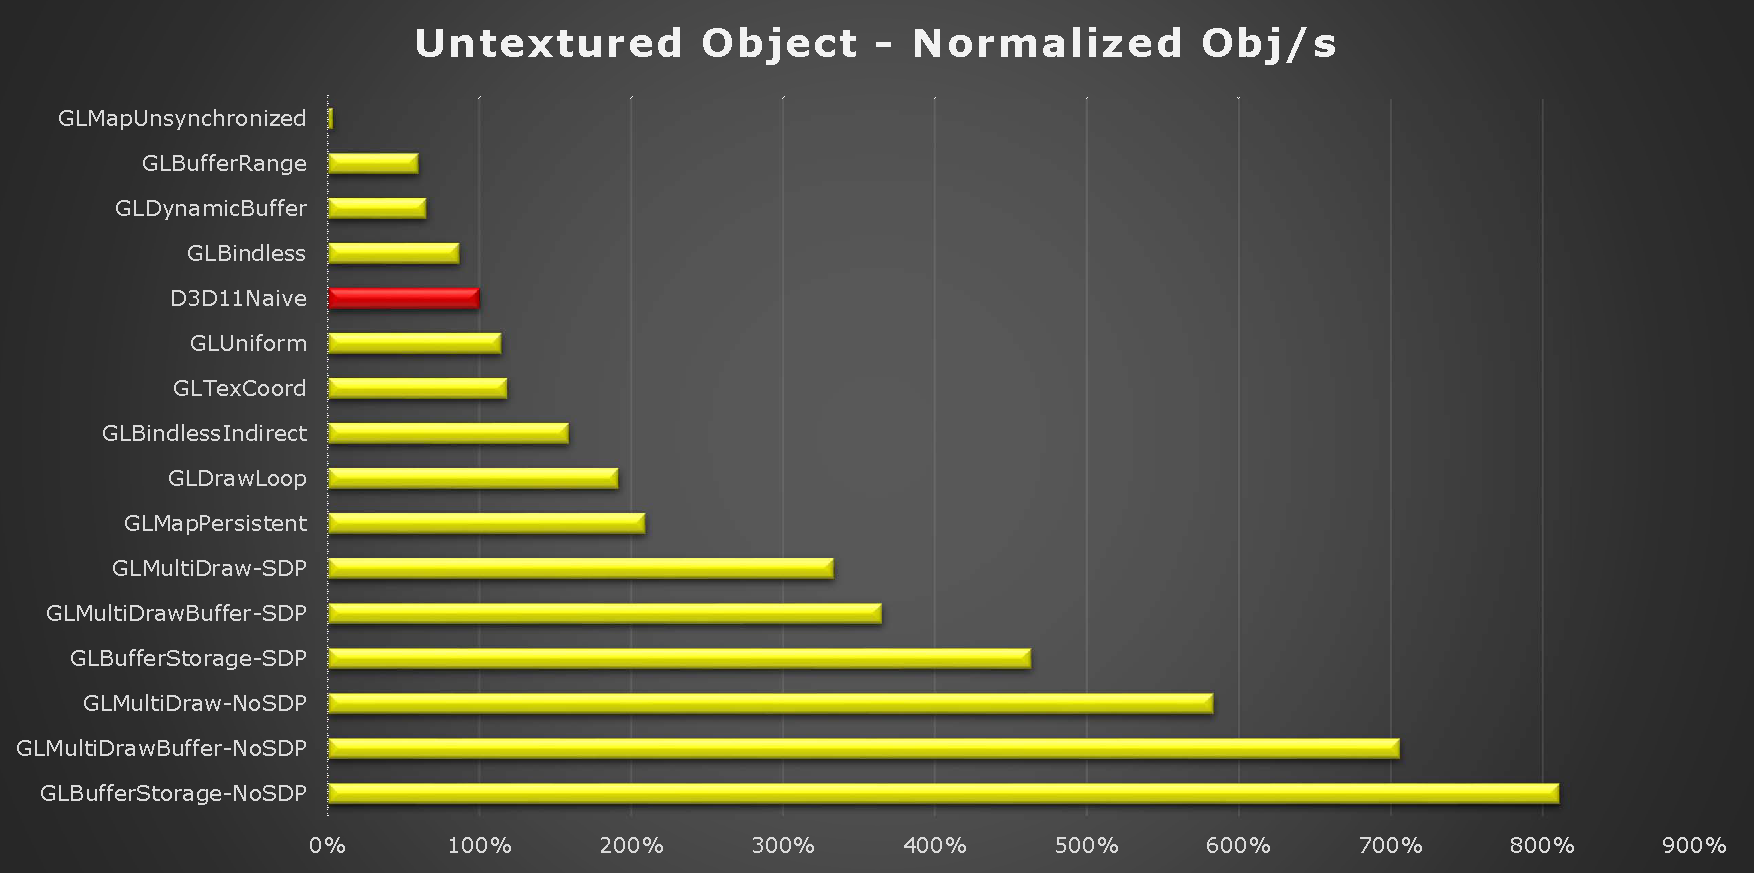
\includegraphics[width=\textwidth]{opengl-spread}
	\caption[Unterschiede in den OpenGL Renderpfaden]{Unterschiede in den OpenGL Renderpfaden \parencite[Seite 98]{Everitt2014}}
	\label{fig:opengl-pfade}
\end{figure}

\paragraph{\acl{MDI}} 
\ac{MDI} beschreibt das Ausführen von mehreren Draw-Calls mit einen API Aufruf. Anstatt für jedes Objekt die notwendigen Aufrufparameter des Draw-Calls separat anzugeben, werden die für alle Objekte notwendigen Parameter in einem OpenGL Buffer (\textit{Command Buffer}) zusammengefasst. Der einzelne indirekte Draw-Call entspricht im wesentlichen nur noch einem Aufruf mit einem Zeiger auf den Inhalt des Command Buffers. Die Parameter können entweder von der CPU aus bestimmt werden oder direkt auf der GPU (z.B. durch View-Frustum Culling auf der GPU). Das Konzept des indirekten Renderns fasst das indexbasierte Rendern und instanziiertes Rendern zusammen\footnote{https://www.opengl.org/wiki/Vertex\_Rendering\#Indirect\_rendering}. Der Command-Buffer in Verbindung mit dem Draw-Call beschreibt ausschließlich die Gestalt des für allen Objekte gemeinsamen \textit{Vertex}-Buffers. Da nun für jedes Objekt kein seperater Draw-Call ausgeführt wird, können auch keine individuellen Daten per Object (zum Beispiel Transformationsmatrizen) an die Shader übergeben werden. Das macht es erforderlich entsprechende Daten gebündelt in einem Array oder \ac{SSBO} dem Shader zu übergeben. Der indizierte Zugriff kann im Shader dann über eingebaute Variablen erfolgen. Dies reduziert zusätzlich den Overhead.

\paragraph{\acl{DSA}} Ein weiterer Schritt zur Reduzierung des Treiber Overheads ist die \ac{DSA} Erweiterung von OpenGL \parencite{Killgard2014} die in den nächsten Jahren mit OpenGL 4.5 Einzug halten wird. Die unterschiedlichen OpenGL Objekte besitzen meistens einen eigenen internen Zustand. Soll dieser Zustand aktualisiert oder abgefragt werden, müssen die Objekte zuvor über Selektoren gebunden werden. Dies ist oft nicht nur fehleranfällig sondern sorgt für wenig intuitiven und lärmenden Quelltext. Zusätzlich erhöht es den API Overhead. 

Mit \ac{DSA} fällt das Selektieren von Objekten vor dem Zugriff auf den Zustand weg und es werden neue Operationen bereit gestellt, die das entsprechende OpenGL Objekt als Parameter erwarten. So lässt sich der Zustand abfragen und manipulieren ohne dass das Objekt vorher im globalen Zustand gebunden werden muss. Dies reduziert den Overhead etwas. Im wesentlichen vereinfacht es die Programmierung mit OpenGL Objekten und erlaubt die Kapselung von Funktionalitäten und erleichtert damit die Umsetzung von komponierbaren Bibliotheken \fref{chap:haskell-modern-gl}.

\paragraph{Separate Program Objects} Auch wenn \ac{DSA} erst mit OpenGL 4.5 breiten Einzug ins \textit{Core} Profil genommen hat, fand die Erweiterung |ARB_separate_program_objects| \parencite{Killgard2011} schon mit Version 4.1 ihren Weg in das \textit{Core} Profil. Zuvor mussten die unterschiedlichen Shader Stufen (Vertex, Geoemetry, Fragment usw.) in ein monolithisches Programm übersetzt werden. Mit der Erweiterung können die einzelnen Stufen unabhängig von einander übersetzt werden. Die Program-Objekte lassen sich dann, unter der Berücksichtungen der Schnittstellen, frei zu einer Programm-Pipeline zusammen setzen. Zusätzlich führt die Erweiterung \ac{DSA} für die Program-Objekte ein, so dass nicht mehr vor der Uniform-Variablenzuwesung die Shader-Objekte gebunden werden müssen. Stattdessen können die Zuweisungen direkt mit dem Program-Objekt durchgeführt werden \warn{link section: \fref{chap:haskell-modern-gl}}.

% ### http://www.g-truc.net/post-0320.html

\section{Vulkan}

\textit{Vulkan} (vormals \textit{glNext}) und \textit{SPIR-V} ist der nächste Schritt (oder Versuch) der \textit{Khronos Group} sich der über Jahrzente gesammelten Altlasten der OpenGL-API zu entledigen. Vulkan wurde im März 2015 als frischer Neustart der Grafik-API angekündigt. Noch ist die Spezifikation am entstehen, aber das erklärte Ziel von Vulkan ist die Reduzierung des CPU Overheads, die breitere Ermöglichung von Multi-Threading und die Abschaffung des impliziten OpenGL Context hin zu einer expliziten API. Neben \textit{Vulkan} wurde \textit{SPIR-V} als eine neue Shader \ac{IL} bzw. Zwischensprache vorgestellt. SPIR-V soll neue Freiräume schaffen eigene Shader-Sprachen sowie Analsyse- und Debuggingtools zu entwickeln\parencite{Olson2015}.

Die Gründe für einen harten Schnitt in der API sind auf zwei Seiten zu suchen. Zum einen ist für den API-Anwender die OpenGL-API wie bereits erwähnt voller Fallstricke. Auf der anderen Seite sind die aktuellen OpenGL Treiber zu einem großen Flickenteppich verkommen. Viele Treiberimplementierungen sind voller Weichen und und Spezialfällen, um bekannte Fehler in der Anwendung der API abzufangen oder potenziell langsame Pfade in schnellere Pfade zu übersetzen \parencite{gamedevnet:glnext}.

\begin{figure}
	\label{fig:microfacet}
	
\includegraphics[width=.5\textwidth]{Vulkan_Mar15}
	
\includegraphics[width=.5\textwidth]{SPIR_Nov14}
	\caption{Vulkan \& SPIR-V}
\end{figure}


